\chapter{はじめに}
\label{chp:first}

\section{はじめに}
\label{sec:paragraph}

3Dプリンターは2010年代に低価格のものが登場するようになってから特に注目をされ続けている.
低価格化が進んだことで一般にも普及が進んでいる.
3Dプリンターを活用することで製造業では,生産過程において開発期間やコストを削減することや素材の選択や高性能化ができる.
特に,これまで大量生産により,均一化された商品が一般的な社会が形成されてきたが,3Dプリンターの登場と普及により多種多様の者を少量生産ずつ,一般家庭で生産することができる.
これまで,生産者と消費者は別の者であったが,3Dプリンターの登場により生産者と消費者が同一の存在となるなりつつあるのだ. 消費者の生産者化により,これまでにない発想の商品が数多く登場し,より便利なこれまでにない発想の商品はデジタル社会により,世界中に拡散され,人類社会の発展に貢献されると考える.
3Dプリンターは人類の可能性を最大化させるためのツールでもある.その3Dプリンターは印刷できる素材が限られているのが現状である.新たな3Dプリンターの素材を開発することは,多くの人が3Dプリンターを使い新しいものを作り出し、人類の想像力を最大化させるうえで重要なことだと考える.


\section{現在の3Dプリンター}
\label{sec:paragraph}

3Dプリンターにはいくつかの種類がある..
主に材料押出法,液槽光重合法,シート積層法,結合剤噴射法,材料噴射法,粉末床溶融結合法,指向性エネルギー堆積法などである.
プリンターに置ける主な機構は図1.1に示す.

\begin{figure}[H]
  \centering
  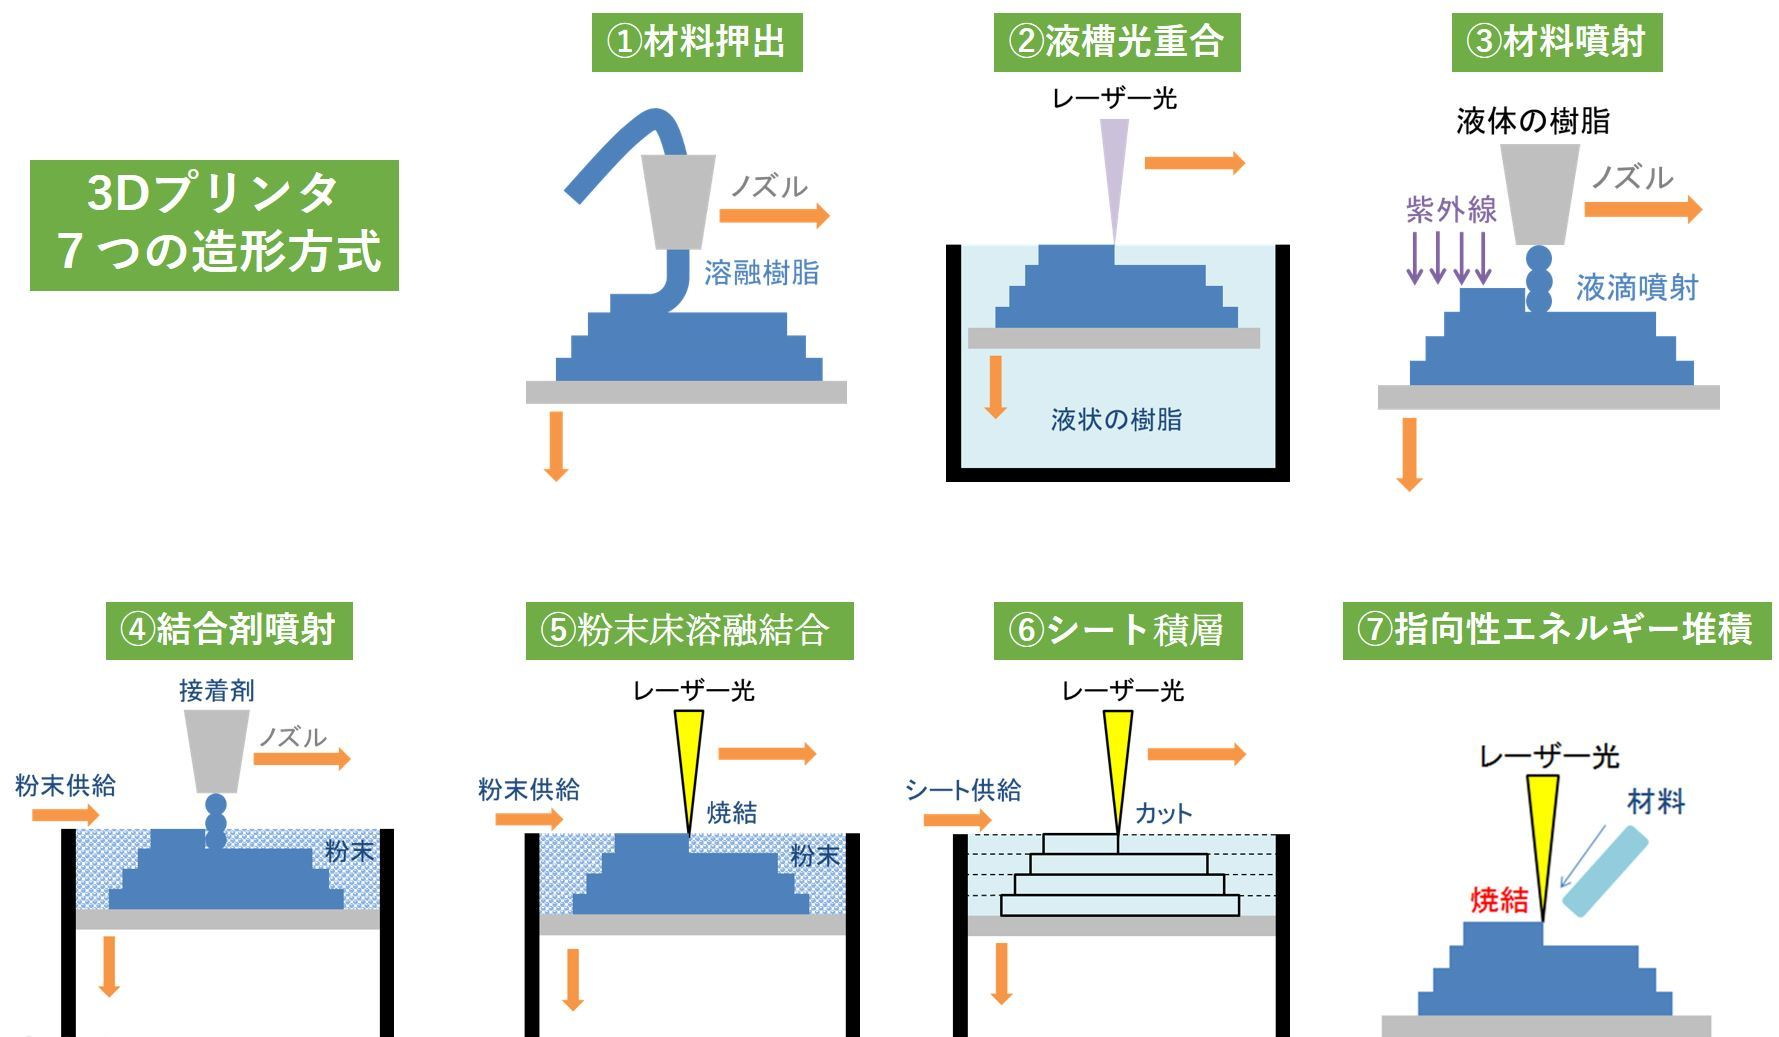
\includegraphics[width=15truecm]{./fig/3Dprinter.jpg}
  \caption{3Dプリンターの造形方法一覧}
  \url{https://monoist.itmedia.co.jp/mn/articles/2007/28/news007.html} % Web上のデータの場合、参照先URLを明記
  \label{fig:ゲル}
\end{figure}

特に一般に普及している3Dプリンターは3種類ある.

材料押出法中でも熱溶解積層方式(FDM)は,ある程度の精度(±0.1~0.2㎜程度)と速度を有し,近年では3万円以下と低価格で一般にもっとも普及している.
機構は,プラスチックのマテリアルを加熱し細いノズルから押し出して層を積み上げ造形物を作る.


液槽光重合法(光造形法(SLA))は,最も古い3Dプリンターの積層方式で,紫外線で硬化する樹脂を使用し積層していく方法である.
一層作るごとに樹脂が固まるまで紫外線を当てるため,造形に時間がかかる,その代わりに精度の高い造形(0.05㎜程度)ができるのが特徴である.
しかし,液槽光重合法(光造形法(SLA))は,マテリアルの樹脂が高価であるとともに,造形後の掃除に手間がかかり,完成後も造形物が完全に硬化するまで紫外線を当て続ける必要がある.


粉末床溶融結合法,なかでもーザー焼結 (SLS) は,金属粉末にレーザーを当て熱で溶かすことにより積層を行う.
レーザーで熱を加えるため時間がかかるが,高い精度でオブジェクトの印刷ができる.
印刷には,金属を溶かすほどの出力の強いレーザーが必要になるためサイズやコスト,安全面を考えても一般家庭では使用が難しいのが現状である.
しかし,鋳造では再現できない,液体を通すことのできる構造を作り出せるため,新しい活用方法も模索されている.


3Dプリンターに重要とされる要素は印刷精度と印刷にかかる時間があると考える.
それぞれのプリンターがどの程度2つの要素を満たしているかを図1.2に示す.
縦の軸が精度を示し,横の軸が印刷にかかる時間を表す.表を見てわかる通り,ある程度普及している3Dプリンターはある程度の造形速度と精度を兼ね備えている.
氷の造形物を印刷するプリンターは,速度を犠牲にして正確な造形物を印刷する業務用タイプのみである程度印刷速度を持ったプリンターが無い.
そこで,私は精度と速度を両立させた氷の3Dプリンターを開発した.現在広く普及しているプリンターの一部を改修することで氷造形を可能にする.

\begin{figure}[H]
  \centering
  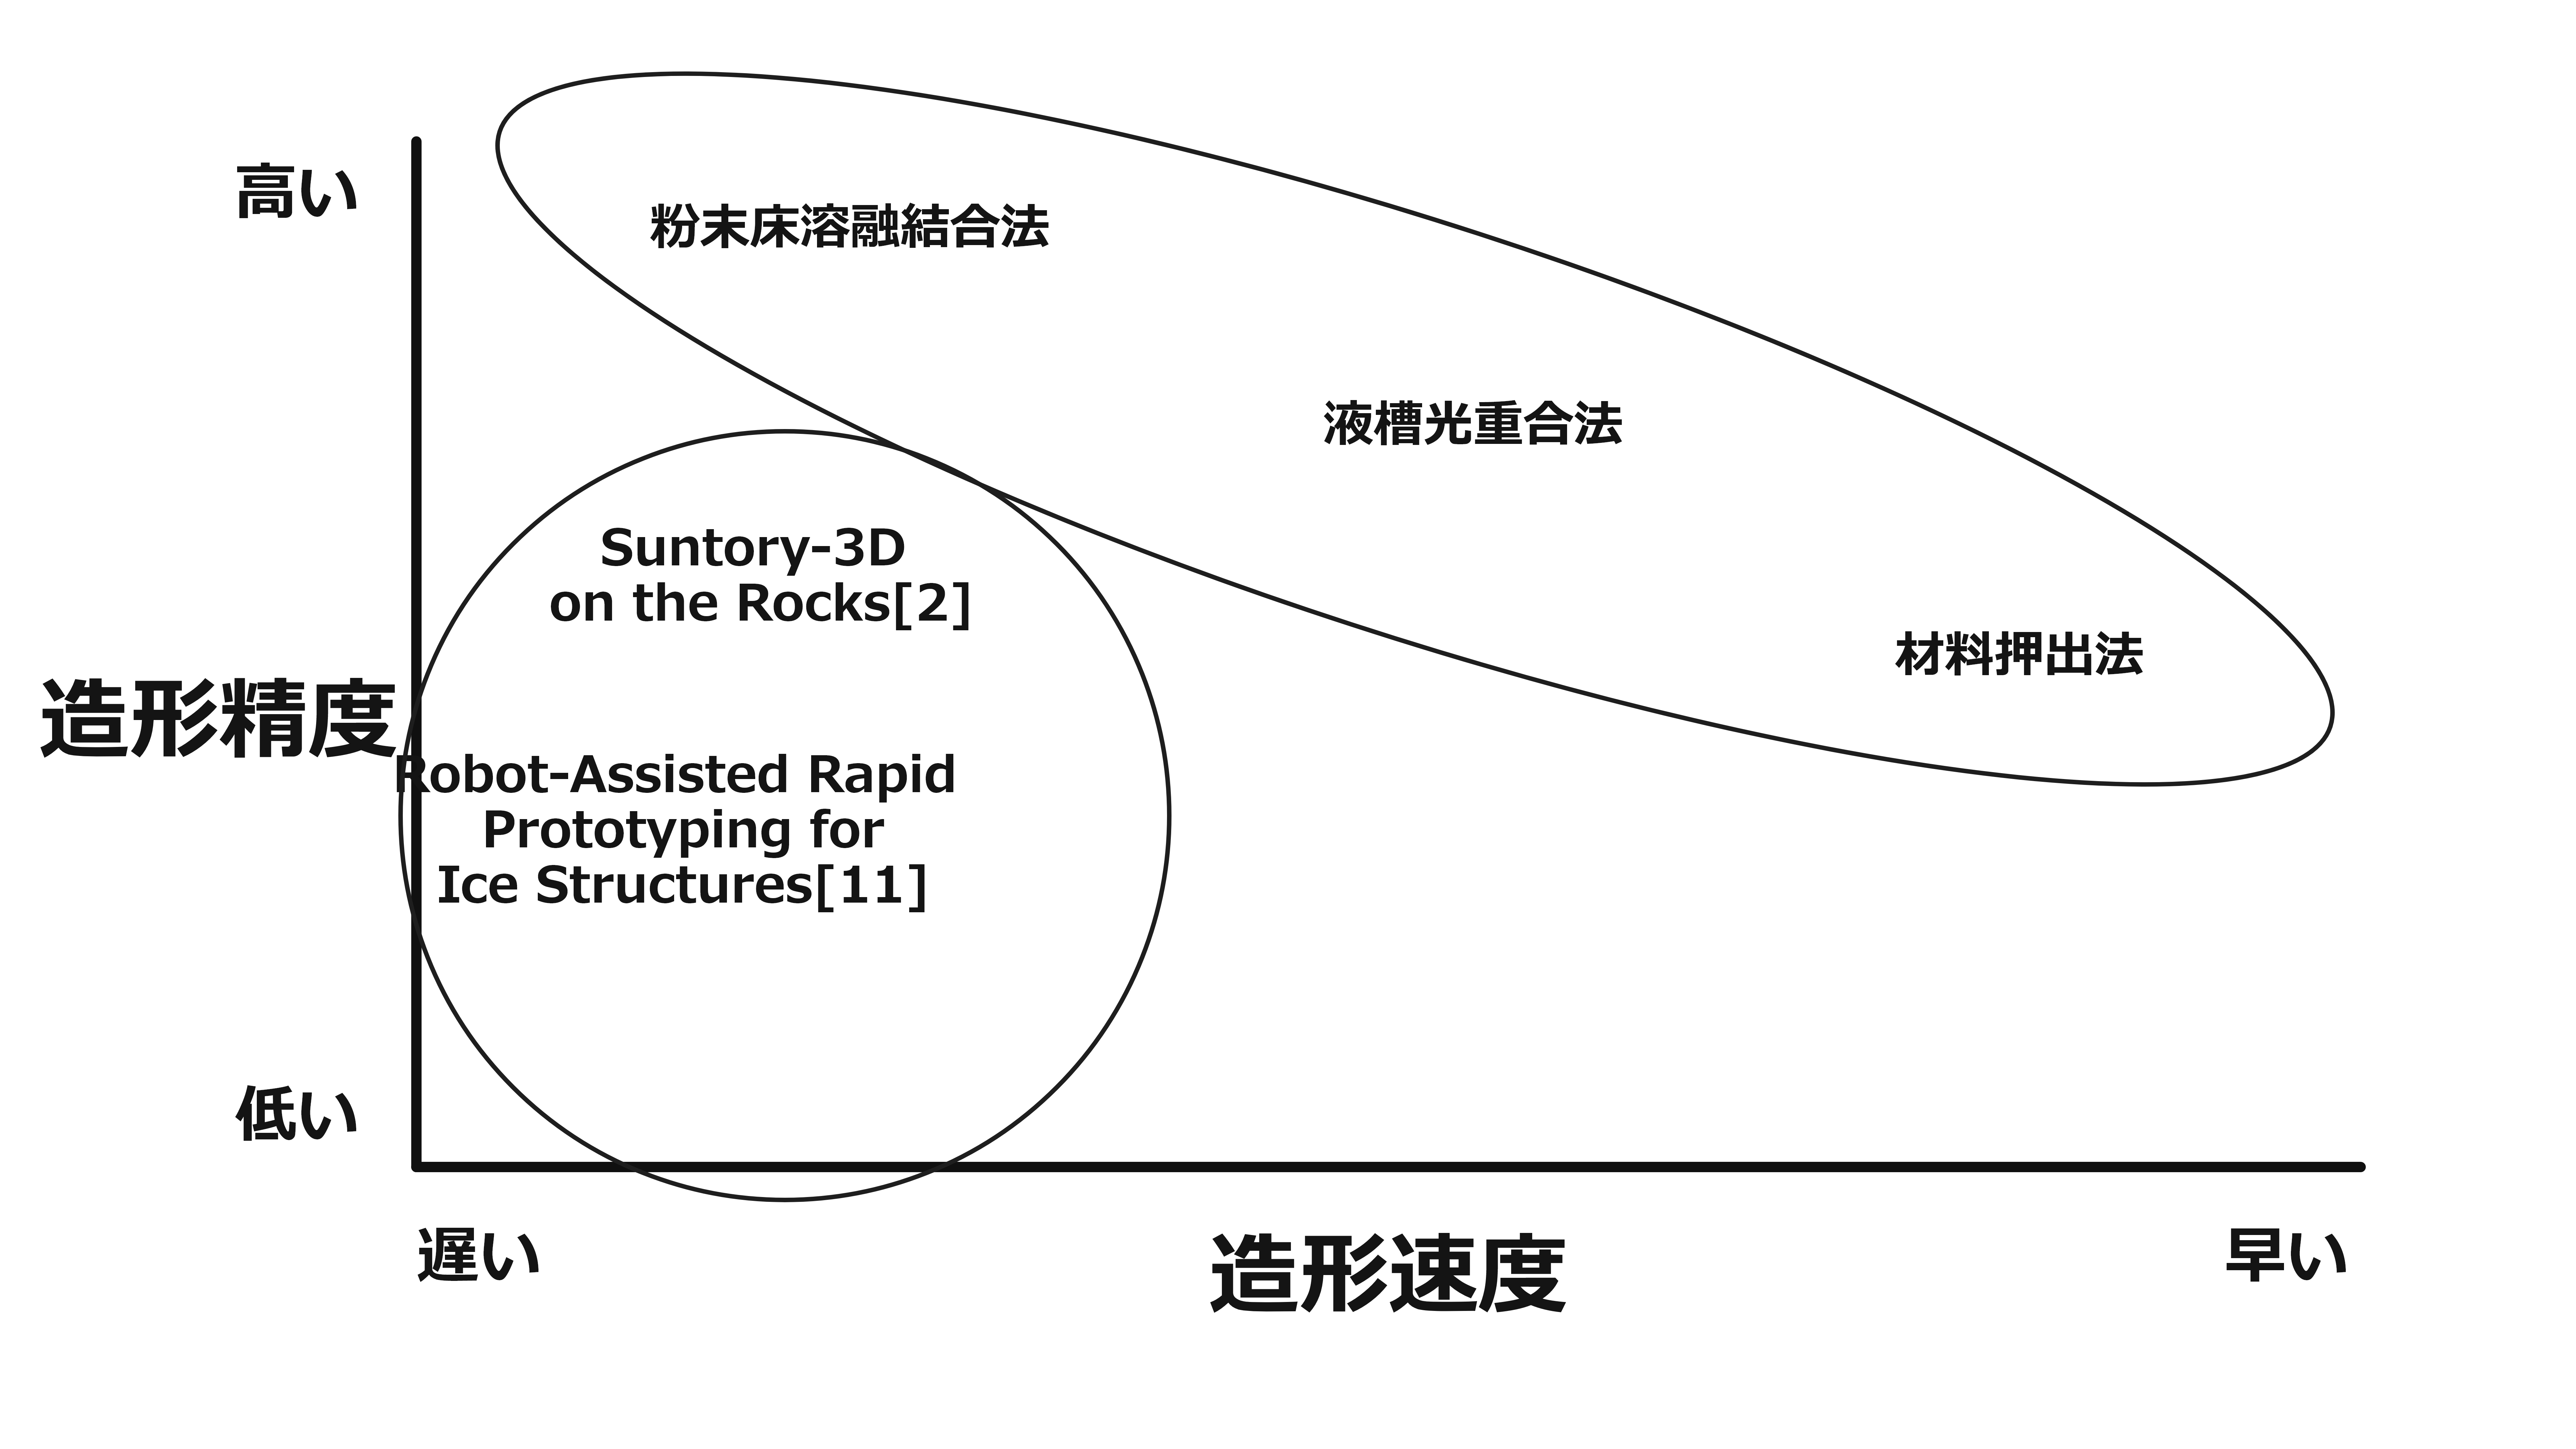
\includegraphics[width=14truecm]{./fig/hyou.jpg}
  \caption{印刷速度と精度の関係}
  %\url{https://idarts.co.jp/3dp/toyamadesign-gp-color-fab/} % Web上のデータの場合、参照先URLを明記
  \label{fig:ferret}
\end{figure}

\section{氷をマテリアルとした3Dプリンター}
\label{sec:paragraph}

氷の彫刻は,世界中で様々なイベントやアート作品に用いられている.
氷は透明なその美しさと時間とともに変化し,最後には溶けてなくなる儚さから人々に親しまれており,様々な作品が作られている.
しかし,誰でも簡単に触れ合えるものではなく,氷の作品を楽しめる場所は限られているのが現状である.
その原因として氷の作品は作るのに時間がかかり,彫刻の技術や設備が必要となる.
私は誰でも簡単に思い通りの形状の氷の作品を作れるようにするため,3Dプリンターを使い氷の造形物をプリントする新しい手法を提案する.
現在の3Dプリンターによる高精度な氷造形は,20mm/h のスピードで高さ 0.1mm の積層をしていく.
この速度で氷の造形物を作るには0度以下の部屋を用意し,造形中は常に造形物の周りを低温に保っておかなければならない.
また,Suntory-3D on the Rocks \cite{b} ではCNCを使った切削のため特殊な機材と知識が必要になるため,だれもが扱えるものではない.
3Dプリンターとして開発されるだけでなく,一般の多くの人に普及させるためには精度を保ちつつ素早く造形でいるプリンターである必要がある.
私は,一般の人でも扱いが可能かつ,一般の3Dプリンターと同程度の速度とある程度の精度を両立した氷をマテリアルとした3Dプリンターの提案する.

\section{氷造形の提案}
\label{sec:enum}

氷の造形物をつくる試みは過去に様々の方法で試されてきた.氷をマテリアルとした自動造形には現状3パターンがある.
1つ目が氷の塊をCNCで掘削する方式である.CNC方式では,精度の高い氷をマテリアルとした造形を行おうことができるのだが,特殊な設備と技術が必要になる.
2つ目が3Dプリンターと同じ仕組みで精度の高い造形物を印刷することができるが,造形速度が20mm/hのスピードで高さ0.1mmの積層とかなり速度がかなり遅い.
3つ目が方に水を流し込み,硬化させる方法である.氷を造形する際に一度型をつくる手間や氷になるまでに数時間と時間が掛かる.
これらの氷をマテリアルとした造形方法では造形速度が遅く,冷凍庫のような特殊な環境が必要になるため,一般の人が気軽に氷をマテリアルとした造形を利用することが難しいのが現状である.
氷をマテリアルとした造形物の使用用途は、現実に氷をマテリアルとした工業製品が無いのを考えると,強度的な問題や常温で溶け出す問題などにより,観賞用に用いられることがほとんどと考えられる.
使用用途が観賞用であると考えた場合、工業用製品に必要な要素が正確性(精度)などに対して,観賞用では,氷の条件を満たしたうえで一般の人でも扱いが可能かつ,一般のユーザーが設計したデータにできるだけ近い形に印刷されれば問題ないと考えられる.
また,氷を再定義する.氷をまたリアルとした3Dプリンターの主な使用用途は観賞と考える.観賞とは,氷特有の常温で液体へと徐々に変化し,最後にはなくなるこの過程が,ほかのマテリアルにはない大きな特徴であるこの部分を指すと考える.
そのため、氷の定義として下記の2つを定義する.

\begin{enumerate}
  \item 固体であるとき常温より低温であること. 
  \item 常温で溶けること.
 \end{enumerate}

氷の定義を以上のようにしたうえで,一般の人でも扱いが可能かつ,一般の3Dプリンターと同程度の速度とある程度の精度を両立した氷をマテリアルとした3Dプリンターの提案する.

